\documentclass{../cpct/ctpro}

\title{ACM 算法实验室 2022 年 12 月月赛题目}
\date{2022 年 12 月 4 日}

\begin{document}

\maketitle
\addproblem{Quento}{1000}{256}{传统}{AgOH}
\addproblem{地铁 \textasciitilde 地铁 \textasciitilde}{1000}{256}{传统}{Algor}
\addproblem{数列 \textasciitilde 数列 \textasciitilde}{1000}{256}{传统}{Algor}
\addproblem{布丁 \textasciitilde 布丁 \textasciitilde}{1000}{256}{传统}{gxust}
\addproblem{排队 \textasciitilde 排队 \textasciitilde}{1000}{256}{传统}{Algor}
\addproblem{背包 \textasciitilde 背包 \textasciitilde}{1000}{256}{传统}{Algor}
\addproblem{Guesslang}{10000}{256}{传统}{Zxilly}
\addproblem{聚会 \textasciitilde 聚会 \textasciitilde}{1000}{256}{传统}{Algor}

\section*{比赛信息}

\ctinfotab{ACM 个人赛}{C/C++,~Python,~Java}{3.5}

\section*{题目概况}

\problemtab

\section*{编译命令}

参见 OJ 帮助

\section*{注意事项}

\begin{itemize}
    \item C/C++ 中函数 \lstinline{main()} 的返回值类型必须是 \lstinline{int},程序正常结束时的返回值必须是 $0$。
    \item C/C++ 代码必须完全符合 GNU C/C++ 标准,不能使用诸如绘图、Win32API、中断调用、硬件操作或与操作系统相关的API。
    \item C/C++ 代码中允许使用 STL 类库。
\end{itemize}

\paragraph*{} 祝大家取得好成绩!


\makeproblem
\section*{题目描述}

Quento 是一个在 $3 \times 3$ 的格子上进行的游戏,每个格子要么是黑色,要么是白色。两个同色的格子不会相邻,且左上角的格子一定为黑色。每个黑色的格子上有一个数字,每个白色的格子上有一个运算符(只能是 \texttt{+} 或 \texttt{-})。我们称上述的 $3 \times 3$ 格子为“Quento 棋盘格”,例如下图就是一个“Quento 棋盘格”:

\begin{center}
    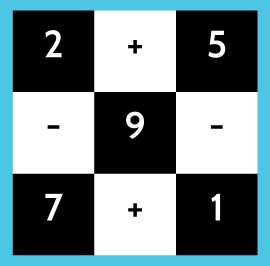
\includegraphics{images/quento.jpg}
\end{center}

Quento 游戏的规则非常简单,给定一个“Quento 棋盘格”,你会获得 $m$ 次询问,每个询问由两个整数 $x_i, y_i$ 组成,你需要回答能否成功进行以下操作:

* 选择一个黑色数字格出发,每步可以向其相邻的格子移动,但不能移动到已经走过的格子,当你到达一个黑色数字格时,你可以选择停止此次移动。把经过的格子上的内容依次写出来会组成一个计算式,你需要使得计算式中数字出现的次数为 $y_i$ 且计算式的结果为 $x_i$。

注意,每次询问是独立的,也就是说你可以移动进一个在其他询问中走过的但当前询问没有走过的格子。

例如,对于上图所示棋盘格,询问 $(11, 2)$ 是可以达成的($9+2=11$):

\begin{center}
    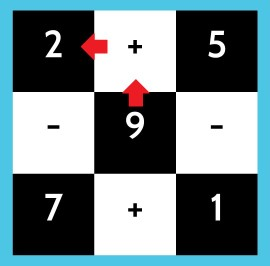
\includegraphics{images/quento1.jpg}
\end{center}

询问 $(3, 3)$ 是可以达成的($9-7+1=3$):

\begin{center}
    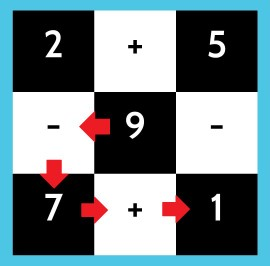
\includegraphics{images/quento2.jpg}
\end{center}

而询问 $(6, 2)$ 则无法达成。

\section*{输入格式}

输入由多个测试用例组成。第一行包含一个整数 $t~(1 \leq t \leq {10}^5)$,代表测试用例的数量。测试用例的描述如下:

前三行,每行三个整数,代表给定的“Quento 棋盘格”。黑色数字格上的整数代表该格子上的数字,保证这个数字的绝对值小于等于 $20$。白色运算符格上的整数只会为 $1$ 或 $-1$:若为 $1$,则代表该格子上的运算符为 \texttt{+};若为 $-1$,则代表该格子上的运算符为 \texttt{-}。

第四行,一个整数 $m~(1 \leq m \leq {10}^5)$,代表询问的数量。

接下来 $m$ 行,每行两个整数 $x_i, y_i~(|x_i| \leq 100,~1 \leq y_i \leq 5)$,代表一次询问。

保证 $\sum m \leq 2 \times {10}^5$。

\section*{输出格式}

对于每个测试用例,对于每个询问,若能够成功进行题目描述所述操作,在一行内输出 \texttt{Yes};否则输出 \texttt{No}。

\section*{输入输出样例}
\testcasetab
{
    2\par
    2 1 5\par
    -1 9 -1\par
    7 1 1\par
    3\par
    11 2\par
    3 3\par
    6 2\par
    5 1 6\par
    -1 7 -1\par
    8 1 3\par
    3\par
    8 3\par
    5 2\par
    -1 5
}
{
    Yes\par
    Yes\par
    No\par
    Yes\par
    No\par
    Yes
}

\section*{说明/提示}

【样例解释】

对于第二个测试用例:

所给“Quento 棋盘格”为:

\begin{center}
    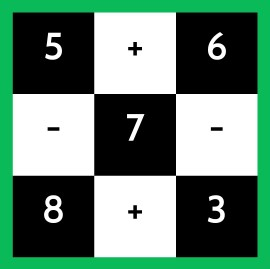
\includegraphics{images/quento3.jpg}
\end{center}

第一个询问可以通过以下方式达成($5+6-3=8$):

\begin{center}
    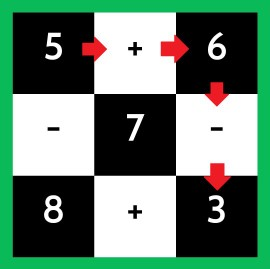
\includegraphics{images/quento4.jpg}
\end{center}

第二个询问不能达成。

第三个询问可以通过以下方式达成($5+6-7-8+3=-1$):

\begin{center}
    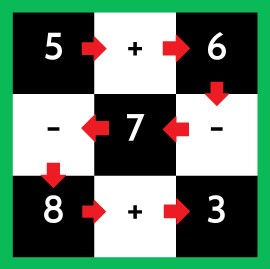
\includegraphics{images/quento5.jpg}
\end{center}

\makeproblem
\section*{题目描述}

$2050$ 年吉安地铁站开通,红苹果幼儿园的小朋友 Algor 迫不及待地拉上了他的小伙伴们一起乘坐地铁去井冈山游玩。由于大家都是第一次乘坐地铁,对于能否到达井冈山心存疑惑,这时社恐的 Algor 决定鼓起勇气向乘务员姐姐询问地铁路线的详情。

Algor 从好心的乘务员姐姐口中得知吉安地铁网络共有 $n$ 个站点(编号从 $1$ 到 $n$),$m$ 条线路,以及每条线路双向连接的两个站点(保证两个站点之间不存在一条以上的线路,一条线路不会连接相同的站点)。

假设 Algor 所在的始发站编号是 $s$,井冈山站的编号是 $t$,由于你是 Algor 的小伙伴当中计算机能力最强的,请你帮助 Algor 确认能否到达井冈山站,如果能,输出 \texttt{YES},否则输出 \texttt{NO}。

\section*{输入格式}

第一行,两个整数 $n,m~(1 \leq n \leq 1 \times {10}^{5},~0 \leq m \leq 2 \times {10}^{5})$,分别表示站点和线路的数量。

第二行,两个整数 $s,t~(1 \leq s,t \leq n)$,分别表示始发站和井冈山站的编号。

接下来 $m$ 行,每行两个整数 $u_i, v_i~(1 \leq u_i,v_i \leq n)$,代表站点 $u_i$ 和 $v_i$ 之间存在一条双向线路。

\section*{输出格式}

一行,如果 Algor 一行人能到达井冈山站,输出 \texttt{YES},否则输出 \texttt{NO}。

\section*{输入输出样例}
\testcasetab
{
    5 4\par
    1 5\par
    1 4\par
    1 5\par
    2 3\par
    4 5
}
{
    YES
}
\testcasetab
{
    5 4\par
    5 3\par
    1 4\par
    1 5\par
    2 3\par
    4 5
}
{
    NO
}

\makeproblem
\section*{题目描述}

你有一个长度为 $n$ 的数列 $A=(A_1,A_2,\dots,A_n)$。

你正好执行了以下操作 $m$ 次:

\begin{itemize}
    \item 删除 $A$ 的首元素并在 $A$ 的尾部追加一个 $0$。
\end{itemize}

在操作之后打印 $A$ 的所有元素。

\section*{输入格式}

第一行,两个整数 $n,m~(1 \leq n \leq 100,~1 \leq m \leq100)$。

第二行,$n$ 个整数 $A_i~(1 \leq A_i \leq 100)$。

\section*{输出格式}

将操作后的 $A$ 的元素打印成一行,用空格分隔。

\section*{输入输出样例}
\testcasetab
{
    3 2\par
    2 7 8
}
{
    8 0 0
}

\section*{说明/提示}

【样例解释】

在操作之前,$A=(2,7,8)$。

执行一次操作后,$A=(7,8,0)$。

进行两次运算后,$A=(8,0,0)$。

因此,$(8,0,0)$ 是答案。

\makeproblem
\section*{题目描述}

宫子从外面带来了 $n$ 块布丁。这些布丁按 $1$ 到 $n$ 进行编号,其中第 $i$ 块布丁的甜度为 $a_i$。

宫子非常喜欢吃布丁,但伊利亚不想让宫子这么快的吃完布丁。因此伊利亚规定宫子每天最多吃 $m$ 块布丁,并且为了帮助宫子锻炼身体,伊利亚安排了惩罚机制。

如果宫子在第 $d$ 天吃了若干块布丁,那么宫子在当天需要做 $y$($y=$ 第 $d$ 天吃掉的所有布丁的甜度总和 $\times~d$)个俯卧撑。

宫子不想做太多的俯卧撑,请你帮助她计算:如果宫子只吃 $x$ 个布丁,她最少要做的俯卧撑总和为多少(从第 $1$ 天到最后一天所做的俯卧撑总和)。

\section*{输入格式}

第一行,两个正整数 $n,m~(1 \leq m \leq n \leq 2 \times {10}^{5})$,分别表示布丁的数量和宫子每天最多能吃的布丁的数量。

第二行,$n$ 个正整数 $a_i~(1 \leq a_i \leq 2 \times {10}^{5})$,表示第 $i$ 个布丁的甜度。

\section*{输出格式}

一行,以空格间隔依次打印 $n$ 个正整数 $res_x~(x=1,2,\dots,n)$,表示如果宫子只吃 $x$ 个布丁,她最少要做多少个俯卧撑。

\section*{输入输出样例}
\testcasetab
{
    9 2\par
    6 19 3 4 4 2 6 7 8
}
{
    2 5 11 18 30 43 62 83 121
}

\makeproblem
\section*{题目描述}

每年的冬天 Algor 都非常想去下海迪土尼玩,今年也不例外。

这天 Algor 和他的小伙伴们来到了下海迪土尼,门口排着长长的队伍,并且队伍参差不齐,机灵的 Algor 立马想到了一个问题:

有 $n$ 个人排成一队,编号从 $1$ 到 $n$,编号较小的人在队伍中的位置更靠前,第 $i$ 个人的身高为 $a_i$,现在 Algor 想知道队伍中有多少对人满足高的排在矮的前面,即求出有多少对 $i,j~(1 \leq i < j \leq n)$ 满足 $a_i > a_j$。

\section*{输入格式}

第一行,一个整数 $n~(1 \leq n \leq 5 \times {10}^{5})$,表示人数。

第二行,$n$ 个整数 $a_i~(1 \leq a_i \leq 1 \times {10}^{9})$,表示第 $i$ 个人的身高。

\section*{输出格式}

一个整数,输出有多少对 $i,j$ 满足条件。

\section*{说明/提示}

【样例解释】

对于所给样例:

第 $1$ 个人身后有 $0$ 个人的身高比他矮;

第 $2$ 个人身后有 $2$ 个人的身高比他矮;

第 $3$ 个人身后有 $2$ 个人的身高比他矮;

第 $4$ 个人身后有 $0$ 个人的身高比他矮;

第 $5$ 个人身后有 $0$ 个人的身高比他矮。

因此答案为 $0+2+2+0+0=4$。

\section*{输入输出样例}
\testcasetab
{
    5\par
    1 3 5 1 2
}
{
    4
}

\makeproblem
\section*{题目描述}

近日,Algor 获得了一个神奇的背包,这个背包可以装下任何重量的物品,唯一的缺陷就是一旦背包内的所有物品的重量总和等于 $m$,背包就会坍缩形成一个黑洞,那将会非常危险。

现在 Algor 想用这个背包来储存他的 $n$ 个金块(编号为 $1$ 到 $n$),由于 Algor 的力量非常小,一次只能往背包中投入一个金块,为了避免世界末日,现在 Algor 来求助你给出一个能将所有金块都放进去的方案。

如果存在这样的方案,则输出它,否则输出 $-1$。

\section*{输入格式}

第一行,两个整数 $n, m~(1 \leq n \leq 1 \times {10}^{5},~1 \leq m \leq 1 \times {10}^{9})$。

第二行,$n$ 个整数 $a_i~(1 \leq a_i \leq 1 \times {10}^{4})$。

\section*{输出格式}

一行,如果存在安全放入所有金块的方案,按照放入顺序输出金块的编号,否则输出 $-1$。

\section*{输入输出样例}
\testcasetab
{
    5 8\par
    1 2 3 4 5
}
{
    1 2 3 4 5
}
\testcasetab
{
    5 15\par
    1 2 3 4 5
}
{
    -1
}

\section*{说明/提示}

如果有多种解决方案,你可以输出任何一种。

\makeproblem
\section*{题目描述}

\texttt{Medise} 写了很多代码,但是她分不清每个代码文件是什么语言的了,你能帮帮她吗?

每个语言有一些关键字,如果一个代码文件中包含了这个语言的关键字,那么这个文件就可能是这种语言。

相同的关键字可能在不同的语言中同时出现。

如果一个代码文件中包含了多种语言的关键字,那么这个文件可能是这些语言中的一种。

例如,\texttt{Python} 语言有关键字 \texttt{def},\texttt{C++} 语言有关键字 \texttt{auto},若一个代码文件的内容为 \texttt{def auto x y},那么这个代码文件就有可能是 \texttt{Python} 或 \texttt{C++} 语言。

\section*{输入格式}

第一行包含四个整数 $m,n,o,p$,表示语言的种数,语言的关键词数,代码文件的数目,以及代码文件中包含的单词数 $(1 \leq m,n,o,p \leq 1000)$。

接下来 $m$ 行,每行以 \texttt{language keyword[...keyword]} 格式给出一个语言的名称和 $n$ 个关键字,语言名称保证不重复,关键字之间用空格隔开。

接下来 $o$ 行,每行包含 $p$ 个字符串,代表一个代码文件的内容。

\section*{输出格式}

对于每个代码文件,输出一行,如果这个代码文件可能是某种语言,那么输出语言的名称,否则输出 \texttt{Unknown}。

如果有多种可能,输出\textbf{字典序最大}的答案。

\section*{输入输出样例}
\testcasetab
{
    3 4 3 3\par
    C int \_Bool if else\par
    Java public static if else\par
    Python def if else yield\par
    if if if\par
    def yield functools\par
    fn export trait
}
{
    Python\par
    Python\par
    Unknown
}

\section*{说明/提示}

【样例解释】

样例中,第一个代码文件中包含了 \texttt{C/Java/Python} 语言的关键字 \texttt{if},所以答案是字典序最大的 \texttt{Python}。

第二个代码文件中包含了 \texttt{Python} 语言的关键字 \texttt{def} 和 \texttt{yield},所以是 \texttt{Python} 语言。

第三个代码文件中不包含任何语言的关键字,所以无法判断是哪种语言。

\makeproblem
\section*{题目描述}

Algor 正在举办一个聚会,他希望聚会上的每一个人都能得到快乐。

他有 $n$ 个朋友,编号从 $1$ 到 $n$,他的第 $i$ 个朋友有 $i$ 块钱。

如果 Algor 邀请第 $i$ 个朋友参加聚会,只有当聚会中最多有 $a_i$ 人严格意义上比他富有,并且最多有 $b_i$ 人严格意义上比他贫穷,他才会快乐。

\section*{输入格式}

第一行,一个整数 $n~(1 \leq n \leq 2 \times {10}^{5})$,表示 Algor 的朋友总数。

接下来 $n$ 行,每行两个整数 $a_i,b_i~(0 \leq a_i,b_i \leq n)$。

\section*{输出格式}

打印 Algor 可以邀请的最大人数。

\section*{输入输出样例}
\testcasetab
{
    3\par
    1 2\par
    2 1\par
    1 1
}
{
    2
}

\section*{说明/提示}

【样例解释】

他邀请了第一个和第二个人。如果他邀请了所有的人,第三个人就会不高兴,因为会有超过 $1$ 个人比他更穷。

\end{document}
